\documentclass[a4paper]{article}
\usepackage[english]{babel}
\usepackage[utf8]{inputenc}
\usepackage{textcomp}
\usepackage{amsmath}
\usepackage{gensymb}
\usepackage{physics}
\usepackage{graphicx}
\usepackage[colorinlistoftodos]{todonotes}
\usepackage{xcolor}
\usepackage{array}
\usepackage{tabularx}
\usepackage{tikz}
\usepackage{framed}
\usepackage{xfrac}
\usepackage[most]{tcolorbox}
\usepackage{fix-cm}
\usepackage[margin=0.5in]{geometry}
\usetikzlibrary{quotes,angles}
\usetikzlibrary{decorations.pathreplacing}
\usetikzlibrary{calc}

\let\phi\varphi
\let\bf\textbf
\colorlet{shadecolor}{orange!15}
\def\centerarc[#1](#2)(#3:#4:#5){\draw[#1] ($(#2)+({#5*cos(#3)},{#5*sin(#3)})$) arc (#3:#4:#5)}

\date{}
\author{}
\title{Week 10 Lecture Notes}

\begin{document}
\maketitle
\section{7/15 Lecture}
\bf{Torque $\boldsymbol{\vec{\tau}}$}
\begin{itemize}
    \item Analogous to force but for rotation
    \item Accelerates rotational motion
    \item Has units of Nm
\end{itemize}
\begin{align*}
    \sum \vec{F}_{net} &= m\vec{a}\\
    \vec{\tau} &= I\vec{\alpha} 
\end{align*}
If there is some net force then there must be some acceleration. $\sum F_{net} \neq 0$
\begin{align*}
    \tau = \vec{r} \times \vec{F} = |r||F|\sin(\phi)
\end{align*}
\begin{align*}
    \vec{A} \times \vec{B} = \vec{C}
\end{align*}

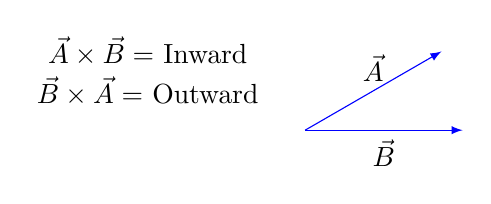
\begin{tikzpicture}[scale= 2]
    \draw[->,draw=blue,-latex] (0,0)--node[below]{$\vec{B}$} (1,0);
    \draw[->,draw=blue,-latex] (0,0)--node[above]{$\vec{A}$} ({cos(30)},{sin(30)});
    \node at (-1,0.5){$\vec{A} \times \vec{B} =$ Inward};
    \node at (-1,0.25){$\vec{B} \times \vec{A} =$ Outward};
\end{tikzpicture}
\begin{align*}
    \vec{A} \times \vec{B} = |\vec{A}||\vec{B}|\sin(\theta)\hat{n}
\end{align*}
Use the right hand rule to determine which direction\\
Anticommutative property: $\vec{A} \times \vec{B} = -\vec{B} \times \vec{A}$\\
The cross product between two parallel vectors is zero

\begin{align*}
    \vec{A} \cdot \vec{B} = |\vec{A}||\vec{B}_{\parallel}| = |\vec{A}_{\parallel}||\vec{B}|\\
    |\vec{A} \times \vec{B}| = |\vec{A}||\vec{B}_{\perp}|
\end{align*}
Comparison of Force and Torque
\begin{align*}
    \vec{F}_{tot} = m\vec{a} = \sum\vec{F}_i\\
    \vec{\tau} = I\vec{\alpha} = \sum\vec{r}_i \times \vec{F}_i
\end{align*}

\begin{shaded}
    \underline{\bf{Example:} Fly Fishing Event}
    \vspace{2mm}\\
    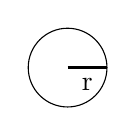
\begin{tikzpicture}
        \draw (0,0) circle (0.5);
        \draw[line width=1pt] (0,0)--node[below]{r}(0.5,0);
    \end{tikzpicture}
    \begin{align*}
        -I_{cm} = \frac{1}{2}MR^2 &= \frac{1}{2}(0.1)(6\times 10^{-2}\text{ m})^2\\
        &= 1.8\times 10^{-4}\text{ kgm}^2\\
    \end{align*}
    \begin{align*}
        I_{cm} &= \frac{1}{2}mr^2\\
        I'_{cm} &= I_{cm} + mR^2\\
        &= \frac{1}{2}mr^2 + mR^2 = 7.3 \times 10^{-5}\text{ kgm}^2 \\
        I_{reel} &= I_{cm} + I'_{cm} = 2.5\times 10^{-4}\text{ kgm}^2
    \end{align*}
    If you apply a force of 200 N tangent to the reel, what is the direction and magnitude of $\vec{\alpha}$:
    \begin{align*}
        \tau = R \times F = |R||F|\sin(90\degree) = I\vec{\alpha}\\
        6\times 10^{-2} \times (200\text{ N}) = 12\text{ Nm}\\
        \alpha = \frac{RFsin(\theta)}{I} = \frac{12}{2.5 \times 10^{-4}} = 4.8 \times 10^{4} rad\;s^{-2}
    \end{align*}
\end{shaded}

\section{7/16 Lecture}
\begin{minipage}{0.45\textwidth}
    \begin{align*}
        \theta\\
        \vec{\omega} = \frac{d\theta}{dt}\hat{n}\\
        \vec{\alpha} = \frac{d\vec{\omega}}{dt}\\
        K_{rot} = \frac{1}{2}I\omega^2\\
        \tau_{tot} = I\vec{\alpha} = \sum \vec{r}_i \times \vec{F}_i
    \end{align*}
\end{minipage}
\begin{minipage}{0.45\textwidth}
    \begin{align*}
        \vec{r}\\
        \vec{v} = \frac{d\vec{r}}{dt}\\
        \vec{a} = \frac{d\vec{v}}{dt} = \frac{d^2\vec{r}}{dt^2}\\
        K_{lin} = \frac{1}{2}mv^2\\
        \vec{F}_{tot} = m\vec{a} = \sum\vec{F}_i
    \end{align*}
\end{minipage}

\begin{shaded}
    \underline{\bf{Example:} Space Telescope}
    \vspace{2mm}\\
    A telescope in outer space is observing some stars. Two air thrusters are each a distance $R$ on either side of the center of mass of the telescope. When the thrusters are activated, each produces a force $F$ in the same direction.
    \begin{enumerate}
        \item[A.] Draw a free body diagram of the telescope, indicating forces acting directly on the mass as a point. Then draw a diagram indicating the placement of the forces relative to the center of mass
        \begin{center}
            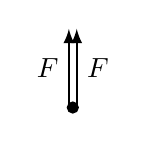
\begin{tikzpicture}
                \filldraw (0,0) circle (2pt);
                \draw[->,-latex,thick] (-0.05,0)--node[left]{$F$}(-0.05,1);
                \draw[->,-latex,thick] (0.05,0)--node[right]{$F$}(0.05,1);
            \end{tikzpicture}
            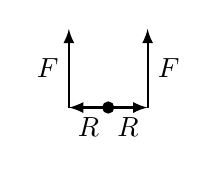
\begin{tikzpicture}
                \filldraw (0,0) circle (2pt);
                \draw[->,-latex,thick] (0,0)--node[below]{$R$}(-0.5,0);
                \draw[->,-latex,thick] (0,0)--node[below]{$R$}(0.5,0);
    
                \draw[->,-latex,thick] (-0.5,0)--node[left]{$F$}(-0.5,1);
                \draw[->,-latex,thick] (0.5,0)--node[right]{$F$}(0.5,1);
            \end{tikzpicture}
        \end{center}
        \item[B.] What is the net force acting on the telescope? What is the net torque around the center of mass?
        \begin{align*}
            \sum F_{net} = F\hat{z} + F\hat{z}\\
            \sum F_{net} = 2F\hat{z}
        \end{align*}
        \begin{align*}
            \sum\tau_{net} = RF\sin(90\degree)\hat{y} + RF\sin(-90\degree)\hat{y}\\
            \sum\tau_{net} = RF\sin(90\degree)\hat{y} - RF\sin(90\degree)\hat{y} = 0
        \end{align*}
        \item[C.] Would the telescope have a linear acceleration? Angular acceleration?
        \begin{center}
            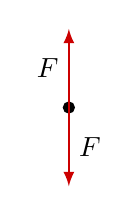
\begin{tikzpicture}
                \filldraw (0,0) circle (2pt);
                \draw[->,-latex,draw=black!20!red,thick] (0,0)--node[left]{$F$}(0,1);
                \draw[->,-latex,draw=black!20!red,thick] (0,0)--node[right]{$F$}(0,-1);
            \end{tikzpicture}
            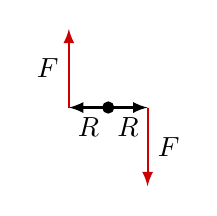
\begin{tikzpicture}
                \filldraw (0,0) circle (2pt);
                \draw[->,-latex,thick] (0,0)--node[below]{$R$}(-0.5,0);
                \draw[->,-latex,thick] (0,0)--node[below]{$R$}(0.5,0);
    
                \draw[->,-latex,draw=black!20!red,thick] (-0.5,0)--node[left]{$F$}(-0.5,1);
                \draw[->,-latex,draw=black!20!red,thick] (0.5,0)--node[right]{$F$}(0.5,-1);
            \end{tikzpicture}
        \end{center}
        \begin{align*}
            \sum F_{net} &= F\hat{z} - F\hat{z}\\
            \sum F_{net} &= 0
        \end{align*}
        \begin{align*}
            \sum\tau_{net} &= RF\sin(90\degree)\hat{y} + RF\sin(90\degree)\hat{y}\\
            \sum\tau_{net} &= 2RF\hat{y}
        \end{align*}
    \end{enumerate}
\end{shaded}

\begin{shaded}
    \underline{\bf{Example:} Acceleration of a Bucket}\\
    \begin{minipage}{0.45\textwidth}
        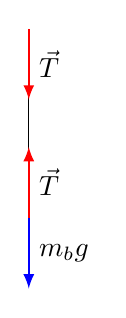
\begin{tikzpicture}[scale=1.5]
            %\draw[<->,dashed,latex-latex] (-1,0)--(1,0);
            %\draw[<->,dashed,latex-latex] (-1,0)--(1,0);
            \draw[line width=0.5pt] (0,1)--(0,-1);
            \draw[->,thick,draw=red,-latex] (0,1)--node[right]{$\vec{T}$}(0,0.4);
            \draw[->,thick,draw=red,-latex] (0,-0.6)--node[right]{$\vec{T}$}(0,0);
            \draw[->,thick,draw=blue,-latex] (0,-0.6)--node[right]{$m_bg$} (0,-1.2);
        \end{tikzpicture}
        \hspace{10mm}
        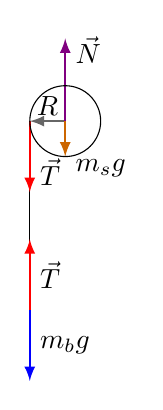
\begin{tikzpicture}[scale=1.5]
            %\draw[<->,dashed,latex-latex] (-1,0)--(1,0);
            %\draw[<->,dashed,latex-latex] (-1,0)--(1,0);
            \draw[line width=0.5pt] (0,1)--(0,-1);
            \draw[->,thick,draw=red,-latex] (0,1)--node[right,yshift=-2mm]{$\vec{T}$}(0,0.4);
            \draw[->,thick,draw=red,-latex] (0,-0.6)--node[right]{$\vec{T}$}(0,0);
            \draw[->,thick,draw=blue,-latex] (0,-0.6)--node[right]{$m_bg$} (0,-1.2);
            \draw[->,thick,draw=black!60,-latex] (0.3,1)--node[above,yshift=-0.6mm]{$R$}(0,1);
            \draw[->,thick,draw=black!20!orange,-latex] (0.3,1)--(0.3,0.7) node[right,yshift=-1.5mm]{$m_sg$};
            \draw[->,thick,draw=violet,-latex] (0.3,1)--(0.3,1.7) node[right,yshift=-1.5mm]{$\vec{N}$};
            \draw (0.3,1) circle (0.3);
        \end{tikzpicture}
    \end{minipage}
    \begin{minipage}{0.45\textwidth}
        \begin{align*}
            F_{net} &= ma\\
            T - m_bg &= m_ba\\
            a &= \frac{T - m_bg}{m_b}
        \end{align*}
    \end{minipage}
    
\end{shaded}

\end{document}